\section{Results}
\label{sec:results}

\subsection{The interface stress field and its decay}
\label{sec:sigma_r}

Figure~\ref{fig:sigma} shows how the stress in the aluminium matrix varies
with the distance $r$ from the interface plane in the two interface cells of
Section~\ref{sec:cell}: the control cell, in which the ridge is unstrained,
and the cell in which the ridge has been elongated by
$\varepsilon=1.94\times10^{-3}$ along the field direction and held there
(Section~\ref{sec:eigenstrain}). The strained cell is built from the relaxed
control by displacing the ridge atoms and is then minimised, so that the two
cells differ in nothing but the strain of the ridge. The matrix is cut into
slices 4~\AA{} thick parallel to the interface, the six components of the
stress tensor are averaged over the aluminium atoms of each slice, and only
then are invariants formed from the averaged tensor
(Section~\ref{sec:stress}). Two averages are used. The first spans the whole
cell in $x$ and $y$, i.e.\ the region above the ridge and the region beside
it; the second is restricted to a window 20~\AA{} wide centred on the ridge
axis, which is the stress that the matrix sees directly above the inclusion.
The ridge---the half-elliptic bump of the inclusion, with semi-axes 35~\AA{}
along $x$ and 20~\AA{} along $z$ (Fig.~\ref{fig:cell})---has its crest at
$r=20$~\AA{}, so that above the crest the distance to the nearest inclusion
surface is $d=r-20$~\AA{}.

\begin{figure}
\centering
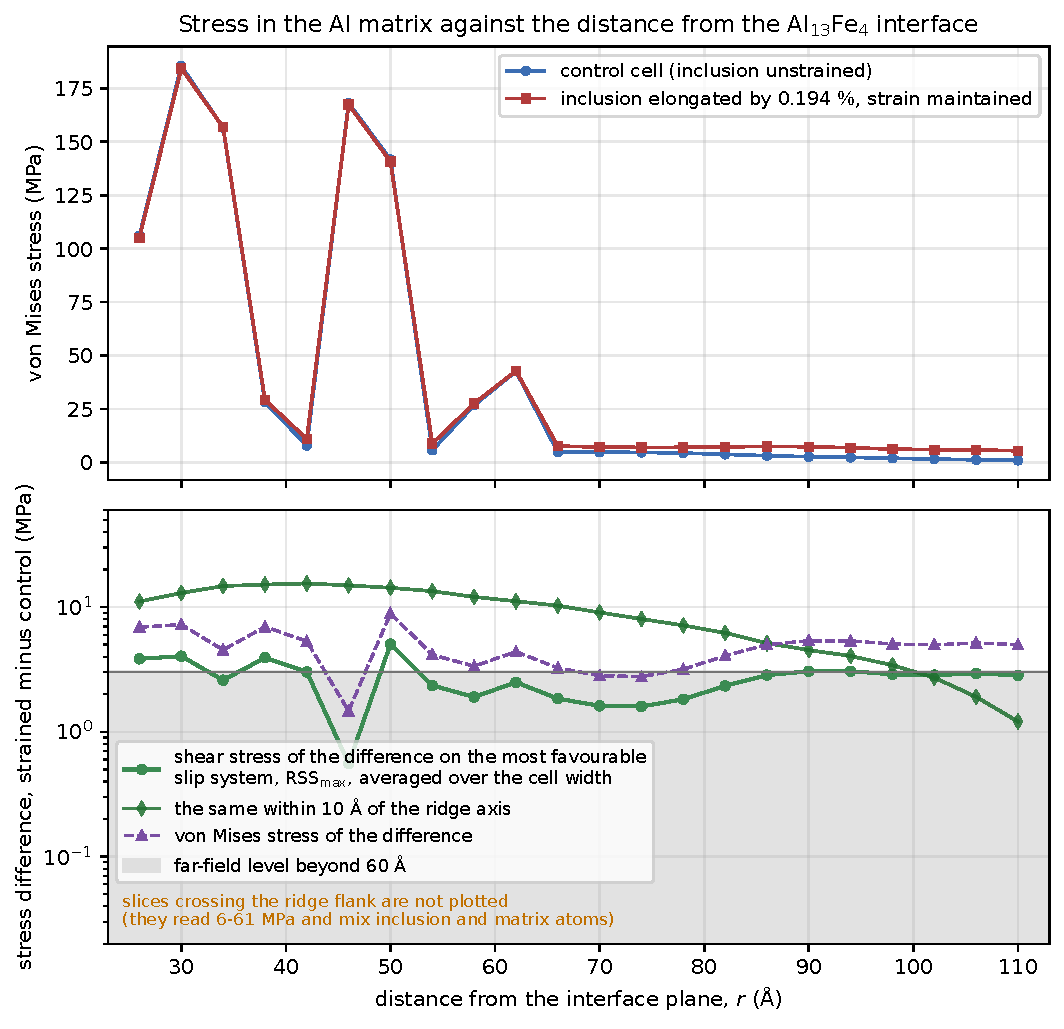
\includegraphics[width=0.85\linewidth]{fig_sigma_profile_en}
\caption{Stress in the aluminium matrix as a function of the distance $r$
from the interface plane in the two interface cells (91\,428 atoms): the
control cell with the unstrained ridge, and the cell in which the ridge is
elongated by 0.194\% along the field direction and held at that strain. The
matrix is cut into slices 4~\AA{} thick parallel to the interface; the six
stress components are averaged over the aluminium atoms of each slice before
any invariant is formed. Top: the von Mises stress in each cell; the
100--190~MPa just above the ridge crest, present in both cells, is the
coherency stress of the bonded interface between two crystals of different
spacing, and the curves coincide. Bottom: the difference
$\Delta\sigma_{ij}=\sigma_{ij}(\varepsilon)-\sigma_{ij}(0)$ as the shear
stress resolved onto the most favourable of the twelve slip systems of fcc
Al, $\mathrm{RSS}_{\max}$, averaged over the whole width of the cell
(circles) and within 10~\AA{} of the ridge axis (diamonds), together with
the von Mises stress of the difference tensor. The shaded region marks stresses below 3~MPa: the width-averaged level
beyond 60~\AA{} with its scatter, $2.5\pm0.5$~MPa, the resolution of the
calculation for long-wavelength strains of the slab. Slices at the level of
the ridge flanks, closer to the interface plane than the crest, are omitted:
there $r$ is not a distance to the inclusion surface and the slices contain
inclusion atoms. The profile ends 20~\AA{} below the free surface of the
slab.}
\label{fig:sigma}
\end{figure}

The upper panel gives the von Mises stress (Section~\ref{sec:stress}) in
each cell. Two features of the control curve need to
be stated plainly, because they are present without any imposed strain.
First, in the slices just above the ridge crest the stress is 100--190~MPa,
and at the level of the ridge flanks it reaches 0.8--2.2~GPa. This is the
coherency stress of the interface. Aluminium and Al$_{13}$Fe$_4$ are
different crystals with different interatomic spacings; across the interface
their atoms interact through the same interatomic potential as inside either
crystal, with no constraint of any kind (Section~\ref{sec:cell}), so the
interface is bonded and cannot slip, and the atoms on both sides are pushed
away from the positions their own lattice would assign them. It falls below
10~MPa beyond $r\approx65$~\AA{} and below 2~MPa beyond about 95~\AA{}; the
alternation between neighbouring slices closer to the crest reflects the
bending of the atomic planes over the crest, where a 4~\AA{} slice holds one
or two planes whose stresses differ. This stress exists whether or not the
ridge is strained: the two curves of the upper panel coincide, the
difference tensor between them having a von Mises stress of at most 9~MPa
above the crest. That is why the effect of the imposed strain is measured
throughout as the difference between the strained and the control cell,
slice by slice. Second, the profile ends 20~\AA{} below the free surface of
the aluminium slab, which lies at $r=129$~\AA{}; in the slices nearer the
surface the per-atom stress is dominated by the surface layers themselves.

The lower panel shows the difference,
$\Delta\sigma_{ij}(r)=\sigma_{ij}(r;\varepsilon)-\sigma_{ij}(r;0)$, which is
the quantity that the mechanism of Ref.~\cite{Friha2024JMMM} requires to
exceed the yield stress of the matrix. Every threshold for dislocation
motion in Section~\ref{sec:thresholds} is a resolved shear stress, so the
difference is expressed in the same way. $\mathrm{RSS}_{\max}$ (Section~\ref{sec:stress}) is computed from the difference tensor, not as a difference of von Mises
values, which would not be an invariant of $\Delta\sigma_{ij}$; the von
Mises stress of the difference tensor is plotted alongside it. In every
slice above the crest but one the most favourable system is
$(111)[1\bar{1}0]$: the
glide plane parallel to the interface and the direction $x$, along which
the dislocations of Section~\ref{sec:thresholds} glide, for which the
resolved shear is simply the component $\Delta\sigma_{xz}$. The exception is
the slice at $r=46$~\AA{}, where the two contributions nearly cancel and the
largest of the twelve values, 0.6~MPa, falls on $(111)[01\bar{1}]$.

Above the ridge axis the resolved shear stress is 11--15~MPa from the crest
out to $d\approx30$~\AA{}, with its maximum of 15~MPa at $d=22$~\AA{}; it
then decays, to 10~MPa at $d=46$~\AA{}, 5~MPa at $d\approx65$~\AA{} and
2~MPa at $d\approx85$~\AA{}. Averaged over the whole width of the cell the
same difference is much smaller, up to 5~MPa (maximum 5.0~MPa at
$r=50$~\AA{}, one slice at 0.6~MPa), because the ridge occupies less than half of the width and
the shear beside the ridge has the opposite sign to the shear above it.
Beyond 60~\AA{} the width-averaged $\mathrm{RSS}_{\max}$ settles at
$2.5\pm0.5$~MPa (mean and standard deviation over thirteen slices). This
level is the resolution of the calculation rather than a field of the
ridge: a uniform shear of 2~MPa across the slab exerts a force of
$10^{-4}$~eV/\AA{} on each atom, below what the minimisation resolves, and
it is with this level that the on-axis field merges at $d\approx80$~\AA{}.
The stress that the strained ridge sends into the matrix is therefore
local: 15~MPa directly above it within one ridge height, and a third of
that on average across a region twice the width of the ridge.

The field is compared in Fig.~\ref{fig:rss} with the exact solution of
Eshelby \cite{Eshelby1957} for a spherical inclusion of the same radius,
35~\AA{}, held at the same strain in an unbounded aluminium matrix: 41~MPa
inside the sphere (47~MPa just outside its surface), 11~MPa at $d=17$~\AA{}, 5~MPa at
$d=35$~\AA{}, falling as the inverse cube of the distance from the centre.
The atomistic ridge produces a smaller stress at its surface and a flatter
profile. The smaller value is a matter of shape: a half-elliptical bump on a
flat layer radiates less into the matrix above it than a compact particle
does (a cylinder holding the same strain carries almost the same interior
stress as the sphere, 39 against 41~MPa); the flatter decay is that of a body
infinite along $y$, whose field falls off more slowly than the inverse cube
of a compact particle. On the ridge axis the two agree within a factor of two between $d=10$ and
$26$~\AA{}. They agree in magnitude only there: closer in the sphere is the
larger, and beyond $d\approx14$~\AA{} the ridge is, until at $d=50$~\AA{} it
exceeds the sphere threefold. The width-averaged curve is not comparable with
either in this way, because slices in which the two contributions nearly
cancel alternate with slices in which they do not. A two-dimensional elastic calculation for the ridge
alone, in an unbounded matrix of the same stiffness, gives 20~MPa at the
ridge surface falling to 5~MPa within 10~\AA{}
(Section~\ref{sec:limitations}). The retained fraction of the imposed
strain, measured by fitting the residual distortion of the Fe sublattice of
the ridge to $\varepsilon^{*}$ (Section~\ref{sec:eigenstrain}), is
$0.97\pm0.004$ in the held cell. When the springs are removed and the inclusion is free to relax, the ridge
retains only 0.2--0.4 of the strain ($0.20\pm0.11$ and $0.44\pm0.10$ in two
minimisations stopped before full convergence) and the shear stress on the
ridge axis falls below 5~MPa; the two free minimisations then also differ across the
whole slab, by $10\pm3$~MPa beyond 60~\AA{} against $2.5\pm0.5$~MPa for the
held pair, because an unconstrained inclusion relaxes along the normal and
shifts the stress of the slab as a whole. The free cell therefore gives the
retained strain but no usable stress field, and the field of
Fig.~\ref{fig:sigma} exists only as long as something holds the inclusion at
its strain.

Slices at the level of the ridge flanks, closer to the interface plane than
the crest, are omitted from the figure. There $r$ measures height above the
interface plane and not the distance to the inclusion surface, which differs
for every atom in the slice; the coherency stress is 0.8--2.2~GPa, and the
difference, 6--61~MPa from one 4~\AA{} slice to the next, mixes the response
of the matrix with the displaced inclusion atoms themselves. These slices
characterise the interface, not the field it sends into the matrix, and they
are not carried forward.

Two qualifications apply. The local stress is deliberately not compared
with the macroscopic yield stress $\sigma_Y\approx120$~MPa: a stress
averaged over a 4~\AA{} slice is not a quantity that can be set against a
yield stress measured on a specimen, and the stresses that matter for
dislocations are measured directly in Section~\ref{sec:thresholds}. Whether
the imposed strain plastifies the matrix is therefore decided by comparing
the difference profile with those measured onsets, not by a local yield
criterion; the interface cells are built without dislocations, and dislocation
analysis of the strained cell after minimisation finds none.
Second, the range of the field---some 30~\AA{} at its full strength and
80~\AA{} in all---is set by the size of the ridge. This accords with a
general property of the Eshelby solution: the stress inside an inclusion
does not depend on its size, whereas the reach of its exterior field scales
with the size \cite{Eshelby1957}, so that a micron-sized inclusion held at
the same strain would carry the same stress over a fraction of a micron---a
point taken up in Section~\ref{sec:bridge}.

\subsection{Thresholds for dislocation activity at the interface}
\label{sec:thresholds}

The stresses at which dislocations respond were measured in the loaded cell
of Section~\ref{sec:loading}, which contains the same ridge together with a
pre-existing pair of edge dislocations of opposite sign (a dislocation
dipole) on glide planes parallel to the interface, under an applied shear
stress rising linearly from 0 to 400~MPa in 96~ps (Fig.~\ref{fig:loading}).
The position of each dislocation was followed frame by frame, every 2~ps, by
dislocation analysis. The onset of motion is defined as the stress at which
the position departs from its thermal oscillation by more than six times the
oscillation amplitude (and by at least 8~\AA{}) and does not return, either
because the line keeps moving or because it ceases to exist. One frame of the
ramp corresponds to 9~MPa, which is the resolution of every onset quoted.

In the control cell, with the ridge unstrained and the inclusion free to
relax during loading, the two partners behave differently from the start. The upper partner sits 32~\AA{} above the crest
of the ridge, in the coherency stress of the interface
(Section~\ref{sec:sigma_r}); it is not at rest at the position where it was
placed and glides 38~\AA{} away from the ridge within the first
6~ps, at zero applied stress, after which it hovers within a few {\aa}ngstr{\"o}ms
of its new position. The lower partner, which by the start of the ramp sits 32~\AA{} beyond the
foot of the ridge, settles by 13~\AA{} in the same interval and then holds. It
starts to move at an applied shear of 95--105~MPa, crosses the
periodic boundary of the cell and within the next 2~ps is no longer
recognised as a dislocation line: it has reacted with the interface. The
upper partner, now unopposed, departs at 115--125~MPa and is
gone in the same way by 180~MPa. No new dislocation appears at the Al/Al$_{13}$Fe$_4$ interface up to the end of the ramp at 400~MPa: heterogeneous nucleation at the interface---the creation of a dislocation at the interface rather than in the perfect lattice---needs more than three times the macroscopic yield stress of the alloy (120~MPa) in this cell. The two do not contradict each other: the yield stress of a specimen reflects the motion of the dislocations it already contains. The only new segments---transiently at 232--241~MPa and again from 377~MPa on---are partial dislocations 10--25~\AA{} long at the periodic boundary of the cell, at the seam left by the insertion of the pair; none is at the interface, and they are a construction artefact.

With the inclusion held by springs, as in the interface cells, the picture
changes in one respect and not in the other. The lower partner is then not
held even at zero applied stress: in the control cell and in the strained
cell alike it is gone by 10~ps, through the periodic boundary,
because the coherency field of a rigidly held, unrelaxed inclusion is
stronger than that of one free to relax. The upper partner moves 31--33~\AA{}
over the ridge in the first 6~ps in both cells, coming to rest 7--10~\AA{}
from its axis, and departs at 105--115~MPa in the control and 115--125~MPa in
the strained cell, one frame of the ramp apart; these two ramps were carried
to 145~MPa, and by 140~MPa the strained cell contains no dislocation while
the control retains only fragments 13--26~\AA{} long at the periodic seam.
A short segment at that seam ($x=7$--$10$~\AA{}, $z=57$--$70$~\AA{}) is
present in both held cells from 12--14~ps on, the same construction
artefact as in the free ramp. The strain of the ridge thus changes the fate
of the pair by at most one frame, 9~MPa. This is the expected result: the
field of the strained ridge at the initial positions of the partners is
5--10~MPa, and on the ridge axis at the height where the upper partner
comes to rest, $d\approx32$~\AA{}, it is 13--14~MPa
(Section~\ref{sec:sigma_r})---both of the order of one frame of the ramp,
so a shift of one frame is neither resolved nor excluded.

The first picoseconds of every ramp, at zero applied stress, answer the question whether the field of the strained ridge alone moves a dislocation placed next to it: the same partner moves in the same way with the ridge strained and unstrained, driven by the coherency field of the interface, not by the strain of the ridge. All onsets are specific to this cell, to the single loading rate
of order $10^{8}$~s$^{-1}$ (relative to quasistatic loading they are upper
estimates), and to the interatomic potential; they are not material
constants. The stress at which the lower partner breaks away,
95--105~MPa, is of the order of the attraction between the two
partners at their separation ($\mu b/[8\pi(1-\nu)h]=198$~MPa for
$h=23.4$~\AA{}, Section~\ref{sec:loading}), reduced by the coherency field
that has already pulled them apart; it lies below the macroscopic yield
stress of the alloy, 120~MPa, because a pre-existing dislocation in a perfect
matrix has nothing but its partner to hold it.

Set against these onsets on the common footing of resolved shear stress, the
stress that the held ridge produces just above its crest, 15~MPa
(Section~\ref{sec:sigma_r}), is a factor of 6--7 below the stress at
which the lower partner starts to move and more than 25 below the highest stress reached without any dislocation forming at the interface (400~MPa), and it falls to
the far-field level within 80~\AA{} of the inclusion. The strained ridge
therefore neither moves the pair nor creates dislocations by itself, and
its bias on the pair is below the resolution of the ramp, one frame or
9~MPa, which is the order of the 5--14~MPa it produces where the pair sits. Figure~\ref{fig:rss} places the
stress profiles and the onsets on one plot.

\begin{figure}
\centering
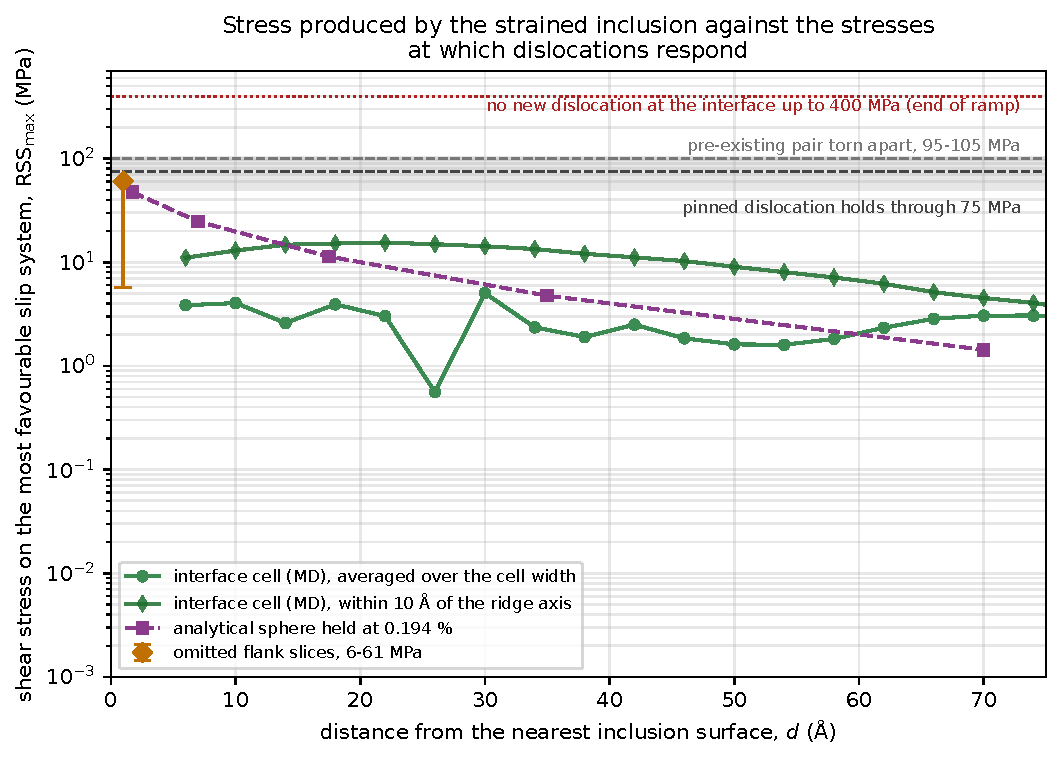
\includegraphics[width=0.9\linewidth]{fig_rss_vs_thresholds_en}
\caption{The stress produced by the strained inclusion against the stresses
at which dislocations respond: the shear stress resolved onto the most
favourable slip system, $\mathrm{RSS}_{\max}$, on a logarithmic scale,
against the distance $d$ from the nearest inclusion surface. Green circles:
the interface cell (91\,428 atoms) with the ridge held at 0.194\%, averaged
over the width of the cell; green diamonds: the same within 10~\AA{} of the
ridge axis; for the ridge $d=r-20$~\AA{} (the crest height). Purple squares:
the exact solution of Eshelby \cite{Eshelby1957} for a spherical inclusion
of radius $a=35$~\AA{} held at the same elongation in an infinite elastic
aluminium matrix ($\mu=26.5$~GPa, $\nu=0.347$, the volume-conserving
elongation of Eq.~(\ref{eq:eigenstrain}) with its axis at $45^{\circ}$ to
$z$, the same maximum over the twelve slip systems); for the sphere
$d=r-a$. Horizontal lines: the end of the ramp, 400~MPa, up to which no new
dislocation formed at the interface (dotted), and the stress at which the
pre-existing dislocation pair starts to move (95--105~MPa), both from
Section~\ref{sec:thresholds}; the shaded band, $75\pm22$~MPa, is the stress
withstood by the pinned dislocation of Section~\ref{sec:mobility} (the
applied 75~MPa, plus or minus the 22~MPa mutual stress of the pair, whose
sign is not resolved). The orange diamond marks the range spanned by the
omitted slices on the ridge flanks; it is not a measurement of the field.}
\label{fig:rss}
\end{figure}

\begin{figure}
\centering
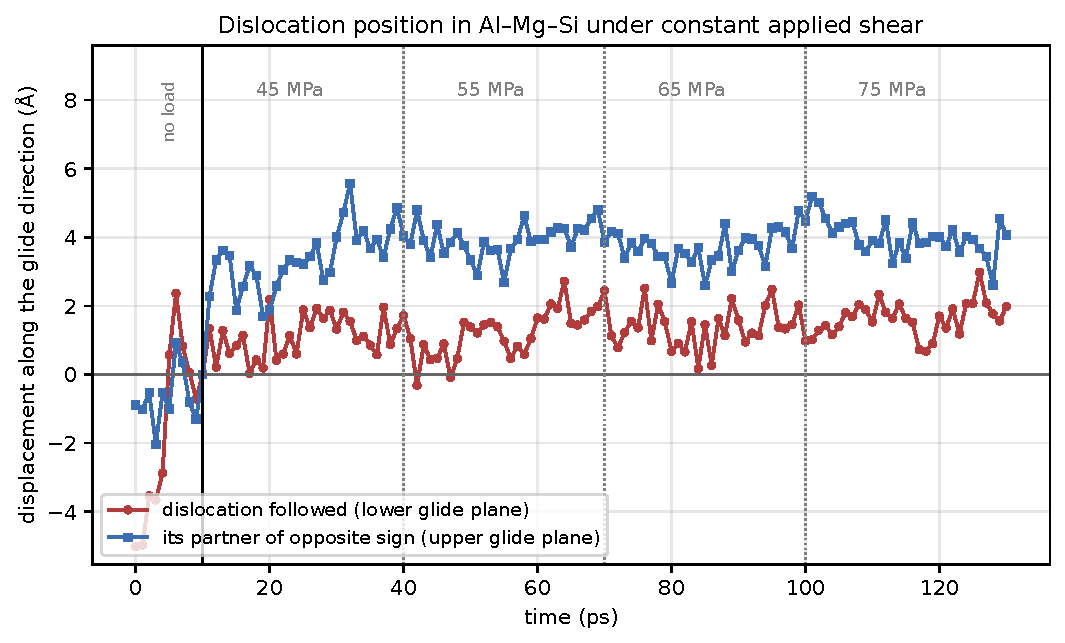
\includegraphics[width=0.9\linewidth]{fig_trajectories_en}
\caption{Position of the dislocation along its glide direction as a function
of time in the Al--Mg--Si cell under the staircase of constant applied shear
stresses (dotted lines: rung boundaries; the applied stress is written above
each rung; the displacement is measured from the position at the moment the load is
switched on, $t=10$~ps, after 10~ps without load). Red: the dislocation whose motion is followed (the
lower member of the pair); blue: its partner of opposite sign on the upper
glide plane. The dislocation oscillates about one position and does not
move: there is no plastic displacement at any of the four stress levels.
Over the whole loading history it advances 2.0~\AA{}, less than one Burgers
vector $b=2.86$~\AA{}, against a thermal oscillation of 0.6~\AA{}. The
partner takes up 4.1~\AA{} ($1.4\,b$) when the load is switched on and then
stops: over the remaining three rungs its position changes by less than its
thermal oscillation of 0.5~\AA{}. That single initial step is not sustained
glide.
}
\label{fig:traj}
\end{figure}

\subsection{Dislocation mobility and solute pinning in the alloy}
\label{sec:mobility}

The resistance that dissolved Mg and Si atoms oppose to dislocation motion
was measured in the alloy cell of Section~\ref{sec:loading}: no inclusion,
1.0~at.\% Mg and 0.6~at.\% Si substituted at random for aluminium, and one
pair of edge dislocations of opposite sign on glide planes 206~\AA{} apart,
loaded by a staircase of constant applied shear stresses of 45, 55, 65 and
75~MPa, 30~ps each. Figure~\ref{fig:traj} shows the position of the
dislocation whose motion is followed (the lower member of the pair) and of
its partner as a function of time. The dislocation does not glide. Over the
120~ps of loading it advances 2.0~\AA{}---less than one Burgers vector
$b=2.86$~\AA{}---against a thermal oscillation of 0.6~\AA{}; the
net displacements within the four rungs, 0.6, 1.6, $-1.5$ and 0.2~\AA{} at
45, 55, 65 and 75~MPa, are comparable to that oscillation and do not grow
with stress. The line oscillates about one position and remains held by the
solute atoms around it at every stress level. A velocity can of course be
fitted to each rung, but at these displacement-to-oscillation ratios
(0.4--2.5) it would measure the oscillation and not a drift, and none is
quoted. What the trajectory does establish is a lower bound: the sampled
random configuration of Mg and Si atoms holds the dislocation against a
driving stress of at least 75~MPa. This exceeds the 15~MPa that the held ridge produces at its
surface (Section~\ref{sec:sigma_r}) by a factor of 5, and the 41~MPa
of the analytical sphere by a factor of 1.8. The two dislocations of the pair
exert a mutual stress of 22~MPa on each other, whose sign relative to the
applied shear is not resolved here, so the conservative reading of the bound
is $75\pm22$~MPa, with a lower edge of 53~MPa, which still exceeds both
amplitudes.
The bound also lies above the Labusch estimate $\tau_c\approx38$~MPa for
this solute content \cite{Labusch1970,Leyson2010}---the mean-field estimate
of the stress needed to drag a dislocation through a random distribution of
solute atoms---which is consistent with a locally stronger-than-average
arrangement of solutes in this single realization.

In the solute-free reference cell of the same geometry the dislocation moves
freely: its position wanders by up to about 20~\AA{} within individual
stress steps, and no trapping event occurs in the 130~ps trajectory. Within
this model, pinning by solute atoms is therefore the only obstacle to
dislocation motion represented in these cells. A quantitative law of
dislocation drag in pure aluminium could not be extracted from the same
geometry: without obstacles one member of the pair reaches the free surface
and is absorbed within the first stress step, and the excursions of the
remaining line are bounded by the residual field of the periodic dislocation
construction; the pinning observation in the alloy is therefore benchmarked
against the Labusch estimate rather than against a measured drag
coefficient. Because no depinning event occurs, the activation volume $V^{*}$ (the volume swept by a dislocation segment as it crosses an obstacle, which sets how strongly the glide rate responds to stress) cannot be extracted from these runs.
The value $V^{*}=70\,b^{3}$ reported by Soula et al.\ for Al--Mg--Si
processed by equal-channel angular pressing \cite{Soula2022JALCOM} is used
as the central case; because that material state differs from the present
one, the range $V^{*}=19$--$142\,b^{3}$ \cite{CaillardMartin2003} is used
only as a sensitivity range. The trajectory serves solely to bound the
obstacle strength from below. No Mg/Si clusters were constructed or identified. A second random
configuration, run only through the 45, 55 and 65~MPa rungs, was likewise
pinned at every rung it reached; the 75~MPa bound rests on the one
realization that completed the staircase.